\documentclass[11pt,a4paper]{article}
\usepackage[T1]{fontenc}
\usepackage[utf8]{inputenc}
\usepackage{lmodern}
\usepackage[margin=22mm,headheight=16pt]{geometry}
\usepackage{amsmath,amssymb,graphicx,array,longtable,booktabs}
\usepackage{microtype,xcolor,hyperref,xurl,fancyhdr}
\definecolor{Navy}{HTML}{17324D}
\definecolor{Teal}{HTML}{087F8C}
\definecolor{Gold}{HTML}{B88128}
\hypersetup{colorlinks=true,linkcolor=Navy,urlcolor=Teal,bookmarksnumbered=true,hypertexnames=false}
\setlength{\parindent}{0pt}
\setlength{\parskip}{6pt}
\setlength{\emergencystretch}{4em}
\setcounter{tocdepth}{1}
\pagestyle{fancy}\fancyhf{}
\fancyfoot[R]{\small\thepage}
\fancyfoot[L]{\small\sffamily Sharif University of Technology}
\renewcommand{\headrulewidth}{0.3pt}
\makeatletter
\renewcommand\section{\@startsection{section}{1}{\z@}{-3.2ex plus -1ex minus -.2ex}{1.6ex plus .2ex}{\normalfont\Large\sffamily\bfseries\color{Navy}}}
\renewcommand\subsection{\@startsection{subsection}{2}{\z@}{-2.5ex plus -1ex minus -.2ex}{1.2ex plus .2ex}{\normalfont\large\sffamily\bfseries\color{Teal}}}
\makeatother
\fancyhead[L]{\small\sffamily\color{Navy}Sharif University of Technology}\fancyhead[R]{\small\sffamily\color{Teal}Project Assignment}\begin{document}
\begin{titlepage}\centering\vspace*{7mm}

\includegraphics[width=31mm]{assets/sharif_emblem_en.png}\par\vspace{5mm}
{\Large\sffamily\bfseries\color{Navy}SHARIF UNIVERSITY OF TECHNOLOGY\par}
\vspace{2mm}{\sffamily Department of Electrical Engineering\par}
\vspace{17mm}{\color{Teal}\rule{\linewidth}{1.4pt}}\par\vspace{6mm}
{\large\sffamily\color{Teal}PROJECT ASSIGNMENT\par}
\vspace{8mm}{\huge\sffamily\bfseries\color{Navy}Folded-Cascode Amplifier Redesign with Class-B Output\par}
\vspace{9mm}{\color{Gold}\rule{45mm}{1pt}}\par\vfill
\begin{minipage}{.88\linewidth}
{\sffamily\color{Teal}INSTRUCTOR / INSTRUCTORS}\par
Dr Mohammad Fakharzadeh; Dr Reza Sarvari; Dr Ali Maddi\par\vspace{7mm}
{\sffamily\color{Teal}ACADEMIC CONTEXT}\par
Electronics II\par\end{minipage}\vfill
\end{titlepage}
\tableofcontents\clearpage
\section{Objective and supplied circuit}

Following the earlier LM741 investigation, design a differential high-gain amplifier and output stage capable of driving a 100-ohm load. Apply feedback to obtain the specified closed-loop gain. Start from the supplied circuit diagram, analyze especially the output stage, identify its limitations, and modify it to meet the design targets. Replace independent sources other than the positive and negative supply rails with appropriate circuits.

\section{Initial analysis: ten required tasks}

\begin{enumerate}

\item Identify input and output stages.

\item Explain Q6 and the bias-current source IB;\allowbreak{} choose IB so Q5 remains on.

\item Calculate transistor operating points and tabulate them.

\item Explain the dead zone expected from class-B output without feedback and how feedback reduces its effect.

\item Calculate output swing and input common-mode range.

\item Identify the mechanisms limiting swing.

\item Simulate in LTspice and show the circuit.

\item Observe node X and the output, comparing the waveforms with the dead-zone analysis.

\item Adjust operating points to increase swing and report the maximum simulated waveform.

\item Define total harmonic distortion and determine it from the simulation.

\end{enumerate}
\begin{figure}[!htbp]\centering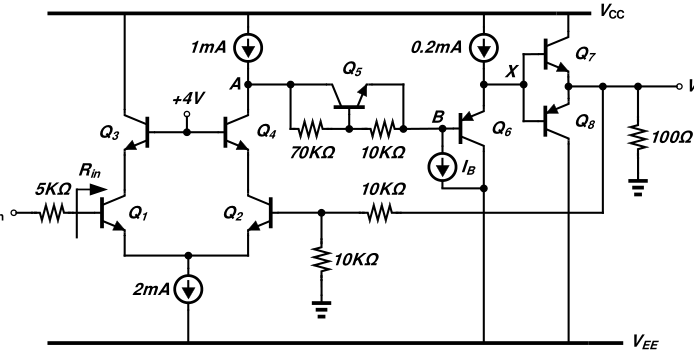
\includegraphics[width=\linewidth,height=.72\textheight,keepaspectratio]{assets/005_p002_vector1.png}\caption{Diagram or recorded result: Initial analysis: ten required tasks.}\label{fig:005_p002_vector10}\end{figure}
\clearpage
\section{Targets and permitted devices}

\begingroup\small\setlength{\tabcolsep}{3pt}\renewcommand{\arraystretch}{1.2}
\begin{longtable}{@{}p{0.4775\linewidth}p{0.4775\linewidth}@{}}
\toprule
\textbf{Requirement} & \textbf{Target} \\ \midrule
\endfirsthead
\textbf{Requirement} & \textbf{Target} \\ \midrule \endhead
Output swing & Greater than 16.6 V peak-to-peak \\
THD & Below 0.05 percent at 16.4 V peak-to-peak \\
Closed-loop gain & 2 \\
Rest/\allowbreak{}quiescent power & At most 50 mW \\
Supplies & +\allowbreak{}10 V and -10 V \\
Transistor count & Fewer than 25 \\
\bottomrule\end{longtable}\endgroup

Use 2N3906-derived PNP transistors with bf=\allowbreak{}150 and 2N3904-derived NPN transistors with bf=\allowbreak{}200, through the specified LTspice model overrides. Only one output-stage transistor may use a different chosen saturation-current parameter while otherwise retaining the permitted model properties.

\section{Redesign tasks}

Draw a folded-cascode input stage, explain its advantages and operating-point selection, and replace the original input with it. Replace all nonsupply sources. In the output stage, replace only current sources with suitable current mirrors;\allowbreak{} additional output-stage changes are prohibited. Input-stage and interstage-level adjustments are allowed. Simulate and show the redesigned circuit. Provide separate evidence for closed-loop gain, output swing, no-input power, and THD at symmetric +\allowbreak{}/\allowbreak{}-8.2-V output. Repeat with the assignment's specified larger feedback resistors and show the output;\allowbreak{} optionally explain the resulting distortion.

\begingroup\small\setlength{\tabcolsep}{3pt}\renewcommand{\arraystretch}{1.18}\begin{longtable}{@{}p{0.4600\linewidth}p{0.4600\linewidth}@{}}
\caption{Redesign tasks - numerical data and parameters.}\label{tab:005_p003_table10}\\\toprule
\textbf{Parameter} & \textbf{Requirement} \\ \midrule\endfirsthead \textbf{Parameter} & \textbf{Requirement} \\ \midrule\endhead
Output swing & Greater than 16.6 V peak-to-peak \\
Total harmonic distortion & Below 0.05\% at 16.4 V peak-to-peak \\
Voltage gain & 2 \\
Quiescent power & 50 mW \\
\bottomrule\end{longtable}\endgroup
\clearpage
\section{Report and files}

Number all figures and tables and cite them in the text. Put figure captions beneath figures and table captions above tables. Include every necessary plot and a full explanation because the report is the grading basis. Work individually. Submit distinct, meaningful filenames for the report and simulation files in an organized ZIP. When design freedom is substantial, state reasonable assumptions and justify choices. Preserve the supplied schematic, operating-point requirements, and target table.

\end{document}